%\setchapterstyle{lines}
%\labpage{appendix}
%\blinddocument
\setchapterpreamble[u]{\margintoc}
\chapter{Appendix}
\section{FluidPaint}
\labsec{fluidpaint}
This section shall explain some of the tricks that were employed to generate a nice-looking data set with \citetitle{fluidpaint}.

The main issue when dealing with this simulation environment is the fact, that control is given over a virtual brush.
This brush has virtual bristles which are necessary to for the simulation.
These bristles introduce an offset between the desired path and the actual path which is colored.\\
Furthermore, these bristles have a momentum and move even when the brush does not paint.
Thus, when moving the brush towards the start point, the bristles will follow the brush.
If the path points into a different direction than the direction the brush just moved in, the bristles will take some time to align along this path.
The result is a kink at the beginning of every brushstroke.
Similarly, if the brushstroke is not followed through afterwards but the brush just stops, then the bristles will move a little further with their momentum and spread out as the brush does not move.\\
Additionally, the brush is reinitialized for every data sample.
Each time the brush is initialized, the bristles can point in random directions which is why the bristles have to be aligned beforehand as well.
\begin{marginfigure}
    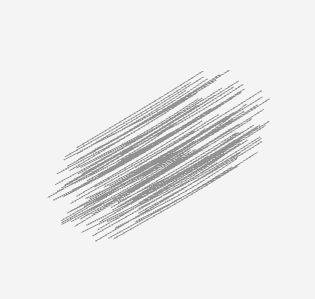
\includegraphics{bristles}
    \caption[]{Image which shows the bristles in \citetitle{fluidpaint}~\cite{fluidpaint}}
    \labfig{linear_class}
\end{marginfigure}

In order to cope with these issues a special ``routine'' is performed with the brush beforehand.
First, the direction at the beginning and at the end of the path are computed.
Then, the brush is moved to the starting point.
There the brush is moved in a circle such that the bristles align.
Thereafter, the brush is moved a bit along the path before it starts painting such that the offset by bristles is compensated.
Now, the brush follows the actual path.
When it reaches the end of the path, it moves a bit longer along the same direction, again to compensate for the length of the bristles.
Finally the brush is moved further along this direction since taking the brush off the canvas takes a few time steps.\\
In the end such a procedure gives brushstrokes that match relatively well with the defined Bézier curve.

It is valid question to ask, why all of this is necessary, as the same offset everywhere would matter much for the parametrization if it is reproducible.\\
Indeed, this is case, although the routine before and after the actual brushstroke would still be necessary to align the bristles.
Thus, is only a little more effort to compensate for the offset that these bristles cause.
Additionally, it helps later on to draw the brushstrokes with other visualization techniques, since the Bézier curves can then be predicted.

\section{Vecotrizing Alpha Blending}
\labsec{alphablend}

The easiest way to accomplish this, is to first find the maximum blending-depth over all pixels, where the blending-depth $k$ is the number of layers where the alpha value is not zero.
\begin{align}
    k = \argmax_{p \in \text{pixels}} \sum_{i \in \# \text{layers}} \mathds{1}(\alpha_i > 0)
\end{align}

Then the top $k$ layer indices for each pixel are picked, which reduces the number of blending operations from $(n-1)$ to $(k-1)$.
Importantly, the top $k$ indices should not be ordered by their alpha values but remain in the order that was imposed by sorting according to the accuracy value.
Otherwise, the order will most certainly be mixed up, and the pixel with the highest alpha value will always lie on top instead of the pixel that belongs to the most accurate brushstroke.
Especially, as brushstroke renderings fade out towards their edges, this makes a significant difference.
Another way of accelerating the process of alpha-blending is \textbf{vectorizing}.
Instead of iteratively applying the computations, a vectorized operation can perform these computations in parallel.
Vectorizing makes it necessary to construct a tensor with the following properties:

For $\tensor{I} \in [0, 1]^{H \times W \times 4} $ the image target, the shape will be defined
as $\mathcal{S}(\tensor{I}) = (H, W, 4)$.
Each alpha channel will have the values $\alpha^{hw} \in [0, 1]$ for $h = 0, ..., H$ and $w = 0, ..., W$.

The set of rendered and padded brushstrokes $\tensor{J}$ will have the shape $(N, H, W, 4)$ with $N$ depicting the number of brushstrokes that ought to be stitched simultaneously.

Now, looking at each individual pixel in $\tensor{J}$, which is described by $(z^{hw}_n, \alpha^{hw}_n)$ for $n = 1, ..., N$ and $z^{hw}_n \in [0, 1]^{3}$, $z^{hw}$ describes the RGB values and $\alpha^{hw}$ the alpha-channel for a pixel at $(h, w)$.

A blending operation can then be defined by
\begin{align}
    z'^{hw} & = \tilde{\alpha}^{hw} \cdot z^{hw} \\
    \text{or} \\
    z'^{hw} & = \sum_{n=1}^N \tilde{\alpha}^{hw}_n  z^{hw}_n \\
\end{align}

with $z'^{hw}$ the resulting RGB values of the blended pixel and $\tilde{\alpha}^{hw}$ a vector that holds the merged alpha values for each pixel:
\begin{align}
    \tilde{\alpha}^{hw} & =
    \begin{pmatrix}
        \alpha^{hw}_1 & &\\
        \alpha^{hw}_2 & (1 - \alpha^{hw}_1) &\\
        \alpha^{hw}_3 & (1 - \alpha^{hw}_2) & (1 - \alpha^{hw}_1)\\
        \vdots & &\\
    \end{pmatrix}
    \\
    & = \alpha^{hw} \odot 
    \begin{pmatrix}
        1  &\\
        (1 - \alpha^{hw}_1) &\\
        (1 - \alpha^{hw}_2) & (1 - \alpha^{hw}_1)\\
        \vdots &\\
    \end{pmatrix}
    \\
    \rightarrow  \tilde{\alpha}^{hw}_n & = \alpha^{hw}_n \prod^{n-1}_{i=1} (1 - \alpha^{hw}_i)
\end{align}

with $\odot$ the element-wise product

What is left, is to find a way to construct $\tilde{\alpha}^{hw}$ from $\alpha^{hw}$.

For this an auxiliary matrix $\beta^{hw}$ is constructed:
\begin{align}
    \beta^{hw} = \alpha^{hw} \times \mathbb{1}_{1 \times N} = 
    \begin{pmatrix}
        \alpha^{hw}_1 & \alpha^{hw}_2 & \hdots & \alpha^{hw}_n\\
        \alpha^{hw}_1 & \alpha^{hw}_2 & \hdots & \alpha^{hw}_n\\
        \vdots & \vdots & \ddots & \vdots \\
        \alpha^{hw}_1 & \alpha^{hw}_2 & \hdots & \alpha^{hw}_n\\
    \end{pmatrix}
\end{align}
with
$$
\mathbb{1}_{1 \times N} = \begin{pmatrix}
        1 \\
        1 \\
        \vdots\\
        1 \\
    \end{pmatrix}^T
$$

Then $\beta^{hw}$ is strictly triangulated such that:
\begin{align}
    \gamma^{hw} & = \beta^{hw} \odot
    \begin{pmatrix}
        0 & 0 & 0 &\hdots & 0\\
        1 & 0 & 0 &\hdots & 0\\
        1 & 1 & 0 &\hdots & 0\\
        \vdots & \vdots & \ddots & \ddots & \vdots \\
        1 & 1 & \hdots & 1 & 0\\
    \end{pmatrix}
    \\ & = 
    \begin{pmatrix}
        0 & 0 & 0 & \hdots & 0\\
        \alpha^{hw}_1 & 0 & 0 & \hdots & 0\\
        \alpha^{hw}_1 & \alpha^{hw}_2 & 0 & \hdots & 0\\
        \vdots & \vdots & \ddots & \ddots & \vdots \\
        \alpha^{hw}_1 & \alpha^{hw}_2 & \hdots & \alpha^{hw}_{n-1} & 0\\
    \end{pmatrix}
    \\
    \rightarrow \delta^{hw} = 1 - \gamma^{hw} & = 
    \begin{pmatrix}
        1 & 1 & 1 & \hdots & 1\\
        (1 - \alpha^{hw}_1) & 1 & 1 & \hdots & 1\\
        (1 - \alpha^{hw}_1) & (1 - \alpha^{hw}_2) & 1 & \hdots & 1\\
        \vdots & \vdots & \ddots & \ddots & \vdots \\
        (1 - \alpha^{hw}_1) & (1 - \alpha^{hw}_2) & \hdots & (1 - \alpha^{hw}_{n-1}) & 1\\
    \end{pmatrix}
\end{align}

By multiplying the elements along each row in $\delta^{hw}$ one gets:

\begin{align}
    \epsilon^{hw}_i = \prod^N_{j=1} \delta^{hw}_{ij} & =
    \begin{pmatrix}
        1  &\\
        (1 - \alpha^{hw}_1) &\\
        \vdots &\\
        \prod^{N-1}_{j=1} (1 - \alpha^{hw}_j)
    \end{pmatrix}
    \\ \rightarrow \tilde{\alpha}^{hw} = \epsilon^{hw} \odot \alpha^{hw} & =
    \begin{pmatrix}
        \alpha^{hw}_1 & &\\
        \alpha^{hw}_2 & (1 - \alpha^{hw}_1) &\\
        \alpha^{hw}_3 & (1 - \alpha^{hw}_2) & (1 - \alpha^{hw}_1)\\
        & \vdots &\\
        \alpha^{hw}_N & \prod^{N-1}_{j=1} (1 - \alpha^{hw}_j)
    \end{pmatrix}
\end{align}

This vectorized version of alpha blending will introduce a new possible bottleneck as it is, since $\beta^{hw}$ will be a tensor of shape $(N, N, H, W)$, which will equate to
$$
256 \times 256 \times 256 \times 256 \times 4 \si{\byte} = 2^{36}\si{\byte} = 64\si{\gibi\byte}
$$
alone.

This is where the previous position-aware alpha blending tricks becomes useful.
By computing $\beta^{hw}$ only through the top $k$ values of $\alpha^{hw}$ instead of the full tensor $\alpha^{hw}$, the size will be reduced to
$$
k \times k \times 256 \times 256 \times 4 \si{\byte} = k^2 2^{22}\si{\byte} = k^2 \times 4\si{\mebi\byte}
$$
as the shape is reduced to $(k, k, H, W)$.

Ultimately, this accelerates optimization by a factor of $2-3$, as it will be shown in \ref{sec:exp:vectorization}.

It must be mentioned that the upper boundary for computational complexity in using this kind of alpha-blending is $\mathcal{O}(N \log k)$, since the top $k$ search is bound by this complexity.
